%\begin{filecontents*}{example.eps}
%!PS-Adobe-3.0 EPSF-3.0
%%BoundingBox: 19 19 221 221
%%CreationDate: Mon Sep 29 1997
%%Creator: programmed by hand (JK)
%%EndComments

%\end{filecontents*}
%
%\documentclass{svjour3}                     % onecolumn (standard format)
%\documentclass[smallcondensed]{svjour3}     % onecolumn (ditto)
\documentclass[12pt,oneside,a4paper]{article}  

\usepackage{apacite}
\usepackage{appendix}
\usepackage{amsmath}
\usepackage{amsthm}
% for ASY interactive 3d figure
\usepackage[inline]{asymptote}
\usepackage{amssymb} % for approx greater than
\usepackage{caption}
\usepackage{placeins} % for \FloatBarrier
\usepackage{graphicx}
\usepackage{subcaption}
\usepackage{longtable}
\usepackage{setspace}
\usepackage{booktabs}
\usepackage{tabularx}
\usepackage{xcolor,colortbl}
\usepackage{chngpage}
\usepackage{natbib}
\bibpunct{(}{)}{,}{a}{}{;} 
\usepackage{url}
\usepackage{nth}
\usepackage{authblk}
\usepackage[most]{tcolorbox}
\usepackage[normalem]{ulem}
\usepackage{amsfonts}

% columns for longtable
%\usepackage{arydshln} % Dashed lines in matrices

\usepackage[margin=1in]{geometry}
%\doublespacing % for review

% line numbers to make review easier
%\usepackage{lineno}
%\linenumbers

%\usepackage{soul}% for \st{}

%%%%%%%%%%%%%%%%%%%%%%%%%%%%%%%%%%%%%%%%%%%%%%%%%%%%%%%%%%%%%%%%%%%%%%%%%%%%%%
% for section 4 math environments
%\theoremstyle{definition}
%\newtheorem{definition}{Definition}[section]
%\newtheorem{theorem}{Theorem}[section]
%\newtheorem{proposition}{Proposition}[section]
%\newtheorem{corollary}{Corollary}[proposition]
%\newtheorem{remark}{Remark}[section]
%
%%%%%%%%%%%%%%%%%%%%%%%%%%%%%%%%%%%%%%%%%%%%%%%%%%%%%%%%%%%%%%%%%%%%%%%%%%%%%%
%\begin{filecontents*}{example.eps}
%!PS-Adobe-3.0 EPSF-3.0
%%BoundingBox: 19 19 221 221
%%CreationDate: Mon Sep 29 1997
%%Creator: programmed by hand (JK)
%%EndComments
%gsave
%newpath
%  20 20 moveto
%  20 220 lineto
%  220 220 lineto
%  220 20 lineto
%closepath
%2 setlinewidth
%gsave
%  .4 setgray fill
%grestore
%stroke
%grestore
%\end{filecontents*}
%\RequirePackage{fix-cm}

\newcommand\ackn[1]{%
  \begingroup
  \renewcommand\thefootnote{}\footnote{#1}%
  \addtocounter{footnote}{-1}%
  \endgroup
}

% Affiliations in small font size
%\renewcommand\Affilfont{\small}
\newcommand{\absdiv}[1]{%
  \par\addvspace{.5\baselineskip}% adjust to suit
  \noindent\textbf{#1}\quad\ignorespaces
}

%\defcitealias{HMD}{HMD 2016}

% junk for longtable caption
%\AtBeginEnvironment{longtable}{\linespread{1}\selectfont}
%\setlength{\LTcapwidth}{\linewidth}

% sort van Raalte properly
% #1: sorting key, #2: prefix for citation, #3: prefix for bibliography
%\DeclareRobustCommand{\VAN}[3]{#2} % set up for citation
%\newcommand{\tc}{\quad\quad\text{,}}
%\newcommand{\tp}{\quad\quad\text{.}}
%%%%%%%%%%%%%%%%%%%%%%%%%%%%%%%
\begin{document}


\title{A note on independant time measures}

%\author{Tim Riffe \and Neil Mehta \and Daniel Schneider \and Mikko Myrskyl\"a}
\author[1]{Tim Riffe\thanks{riffe@demogr.mpg.de}}
\author[2]{Joel Cohen}


\affil[1]{Max-Planck-Institute for Demographic Research}
\affil[2]{The Rockefeller University}


%\authorrunning{Short form of author list} % if too long for running head

\maketitle

\vspace{-2em}
\begin{abstract}
\absdiv{Background} There are countless Lexis-like relationships between
linearly dependant time measures, and these can be combined into higher-order
Lexis identities with dense linear interdependencies. One such relationship is
the demographic time identity between age, period, cohort, time to death, length of life, and time of death. Certain subsets of time measures in this
and other higher order identities consist in time measures that are independant
of one another.
\absdiv{Objective} We aim to describe the relationship between
independent time measures and the identities within which they are nested, with
special attention to the demographic time identity and its three independant
time dyads. We aim to determine whether data structured on such time dyads might
be useful in demographic research.
\absdiv{Data and Methods} We illustrate concepts visually based on data from the
Colonial Qu\'{e}bec Population Register.
\absdiv{Results} 
\absdiv{Conclusions}
\end{abstract}

\section{Geometric relationships}
The demographic time identity maps to the edges of a tetrahedron. When extended
into three dimensions, the tedtrahedron tesselates with octahedra in a 2:1
ratio. In its original description \citep{riffe2017demographictime}, neither
independant pairs of time measures nor the significance of octahedra in this
geometric construct were considered in any depth. Figure~\ref{fig:tet}
shows the tetragedral graph of the demographic time identity between age
(A), period (P), cohort (C), time to death (T), death cohort (D), and length
of life (L). Independant dyads are those that do not share any vertex in the
graph, and these appear already as perpendicular but disjoint in the present
graph representation: CT, LP, and AD.

\begin{figure}[h!]
\centering
\caption{Tetrahedral graph of demographic time hexad identity, with edges
labelled by the six time indices. Reproduced from 
\citet{riffe2017demographictime}.}
\label{fig:tet}
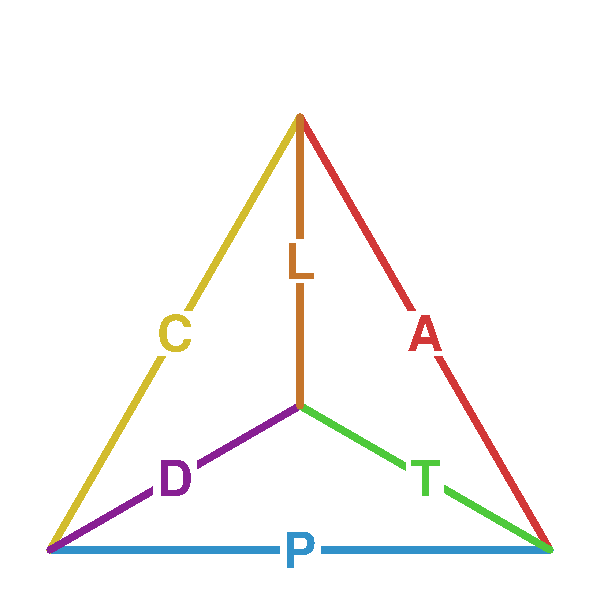
\includegraphics[width=4in]{Figures/TetraHedronEdgesOnly.pdf}%
\end{figure}

As with any arbitrary pair of quantitative variables, independant
temporal dyads can define a standard Cartesian plane. Such planes are
already an isometric projection, and these planes can also represent cross-sections of a 3d demographic time space. The independant planes can also
be conceived of a angles of view on the demographic time space. 

\subsection{View axes}
An angle of view directly at any of the four faces of the demographic
time tetrahedron reveals the plane-perspective defined by one of the
Lexis-like identities.\footnote{In other words, set the viewing axis as
\emph{normal} to one of the faces of the plane.} These four view axes map to
the four medians of a tetrahedron, depicted in Figure~\ref{fig:depviewaxes}
with cyan lines.
Independant dyad planes are revealed when the viewing angle is such that the midpoints of opposite tetrahedral edges are aligned. There are three pairs of
opposite edges (LP, TC, AD), and therefore three viewing angles of this kind.
These map to the bimedians of the tetrahedron, depicted in
Figure~\ref{fig:indepviewaxes} with magenta lines. 

\begin{figure}
\begin{subfigure}{.5\textwidth}
\begin{asy}
// DepViewAxes produced by rgl
settings.prc = true;
size(3inches, 3inches);
import graph3;
currentprojection = orthographic(0, -3.101144, 1.128724, up = (0, 0.3420201, 0.9396926));
defaultpen(fontsize(14));
ticklabel RGLstrings(real[] at, string[] label)
{
  return new string(real x) {
    int i = search(at, x);
    if (i < 0) return "";
    else return label[i];
  };
}

ticklabel RGLScale(real s)
{
  return new string(real x) {return format(s*x);};
}
currentlight = light(ambient=new pen[] {rgb(1,1,1)},
diffuse = new pen[] {rgb(1,1,1)},
specular = new pen[] {rgb(1,1,1)},
position = new triple[] {(0,0,1)},
viewport = true);
currentpen += linewidth(4);
currentpen = colorless(currentpen) + rgb(0.1921569, 0.5686275, 0.7882353);
draw((0.4985029, 0, -0.1762474)
--(-0.2492514, 0.4317162, -0.1762474)
);
label("P", position = (-0.002741766, 0.3181748, -0.1938721), align = (0,0));
currentpen = colorless(currentpen) + rgb(0.8235294, 0.7372549, 0.1764706);
draw((0.4985029, 0, -0.1762474)
--(-0.2492514, -0.4317162, -0.1762474)
);
label("C", position = (-0.002741766, -0.3181748, -0.1938721), align = (0,0));
currentpen = colorless(currentpen) + rgb(0.5333334, 0.1215686, 0.5764706);
draw((0.4985029, 0, -0.1762474)
--(0, 0, 0.5287422)
);
label("D", position = (0.1809565, 0, 0.3257052), align = (0,0));
currentpen = colorless(currentpen) + rgb(0.8235294, 0.2156863, 0.2156863);
draw((-0.2492514, 0.4317162, -0.1762474)
--(-0.2492514, -0.4317162, -0.1762474)
);
label("A", position = (-0.2741766, -0.1614619, -0.1938721), align = (0,0));
currentpen = colorless(currentpen) + rgb(0.3058824, 0.7882353, 0.2313726);
draw((-0.2492514, 0.4317162, -0.1762474)
--(0, 0, 0.5287422)
);
label("T", position = (-0.09047827, 0.156713, 0.3257052), align = (0,0));
currentpen = colorless(currentpen) + rgb(0.772549, 0.4588235, 0.1686275);
draw((-0.2492514, -0.4317162, -0.1762474)
--(0, 0, 0.5287422)
);
label("L", position = (-0.09047827, -0.156713, 0.3257052), align = (0,0));
currentpen += linewidth(2);
currentpen = colorless(currentpen) + rgb(0, 1, 1);
draw((0, 0, 0.6873648)
--(0, 0, -0.2291216)
);
currentpen = colorless(currentpen) + rgb(0, 0, 0);
label("APC", position = (0, 0, -0.2291216), align = (0,0));
currentpen = colorless(currentpen) + rgb(0, 1, 1);
draw((-0.3240269, -0.561231, -0.2291216)
--(0.108009, 0.187077, 0.07637387)
);
currentpen = colorless(currentpen) + rgb(0, 0, 0);
label("TPD", position = (0.108009, 0.187077, 0.07637387), align = (0,0));
currentpen = colorless(currentpen) + rgb(0, 1, 1);
draw((-0.3240269, 0.561231, -0.2291216)
--(0.108009, -0.187077, 0.07637387)
);
currentpen = colorless(currentpen) + rgb(0, 0, 0);
label("CDL", position = (0.108009, -0.187077, 0.07637387), align = (0,0));
currentpen = colorless(currentpen) + rgb(0, 1, 1);
draw((0.6480538, 0, -0.2291216)
--(-0.2160179, 0, 0.07637387)
);
currentpen = colorless(currentpen) + rgb(0, 0, 0);
label("TAL", position = (-0.2160179, 0, 0.07637387), align = (0,0));
currentlight.background = rgb(0.2980392, 0.2980392, 0.2980392);
currentlight.background = rgb(1, 1, 1);
currentlight.background = rgb(1, 1, 1);
\end{asy}

\caption{The four view axes of the triad dependencies map to the medians of the
tetrahedron.}
\label{fig:depviewaxes}
\end{subfigure}
\begin{subfigure}{.5\textwidth}
\begin{asy}
// IndepViewAxes produced by rgl
settings.prc = true;
size(3inches, 3inches);
import graph3;
currentprojection = orthographic(0, -2.640817, 0.9611788, up = (0, 0.3420201, 0.9396926));
defaultpen(fontsize(14));
ticklabel RGLstrings(real[] at, string[] label)
{
  return new string(real x) {
    int i = search(at, x);
    if (i < 0) return "";
    else return label[i];
  };
}

ticklabel RGLScale(real s)
{
  return new string(real x) {return format(s*x);};
}
currentlight = light(ambient=new pen[] {rgb(1,1,1)},
diffuse = new pen[] {rgb(1,1,1)},
specular = new pen[] {rgb(1,1,1)},
position = new triple[] {(0,0,1)},
viewport = true);
currentpen += linewidth(4);
currentpen = colorless(currentpen) + rgb(0.1921569, 0.5686275, 0.7882353);
draw((0.5820827, 0, -0.2057973)
--(-0.2910413, 0.5040984, -0.2057973)
);
label("P", position = (-0.003201455, 0.3715205, -0.226377), align = (0,0));
currentpen = colorless(currentpen) + rgb(0.8235294, 0.7372549, 0.1764706);
draw((0.5820827, 0, -0.2057973)
--(-0.2910413, -0.5040984, -0.2057973)
);
label("C", position = (-0.003201455, -0.3715205, -0.226377), align = (0,0));
currentpen = colorless(currentpen) + rgb(0.5333334, 0.1215686, 0.5764706);
draw((0.5820827, 0, -0.2057973)
--(0, 0, 0.6173919)
);
label("D", position = (0.211296, 0, 0.3803134), align = (0,0));
currentpen = colorless(currentpen) + rgb(0.8235294, 0.2156863, 0.2156863);
draw((-0.2910413, 0.5040984, -0.2057973)
--(-0.2910413, -0.5040984, -0.2057973)
);
label("A", position = (-0.3201455, -0.1885328, -0.226377), align = (0,0));
currentpen = colorless(currentpen) + rgb(0.3058824, 0.7882353, 0.2313726);
draw((-0.2910413, 0.5040984, -0.2057973)
--(0, 0, 0.6173919)
);
label("T", position = (-0.105648, 0.1829877, 0.3803134), align = (0,0));
currentpen = colorless(currentpen) + rgb(0.772549, 0.4588235, 0.1686275);
draw((-0.2910413, -0.5040984, -0.2057973)
--(0, 0, 0.6173919)
);
label("L", position = (-0.105648, -0.1829877, 0.3803134), align = (0,0));
currentpen += linewidth(2);
currentpen = colorless(currentpen) + rgb(1, 0, 1);
draw((-0.436562, 0, -0.308696)
--(0.436562, 0, 0.308696)
);
currentpen = colorless(currentpen) + rgb(0, 0, 0);
label("AD", position = (-0.4656661, 0, -0.3292757), align = (0,0));
currentpen = colorless(currentpen) + rgb(1, 0, 1);
draw((-0.218281, 0.3780738, 0.308696)
--(0.218281, -0.3780738, -0.308696)
);
currentpen = colorless(currentpen) + rgb(0, 0, 0);
label("TC", position = (-0.2328331, 0.4032787, 0.3292757), align = (0,0));
currentpen = colorless(currentpen) + rgb(1, 0, 1);
draw((-0.218281, -0.3780738, 0.308696)
--(0.218281, 0.3780738, -0.308696)
);
currentpen = colorless(currentpen) + rgb(0, 0, 0);
label("LP", position = (-0.2328331, -0.4032787, 0.3292757), align = (0,0));
currentlight.background = rgb(0.2980392, 0.2980392, 0.2980392);
currentlight.background = rgb(1, 1, 1);
currentlight.background = rgb(1, 1, 1);
\end{asy}

\caption{The three view axes of independant dyads map to the bimedians of the
tetrahedron.}
\label{fig:indepviewaxes}
\end{subfigure}
\caption{The seven principal view axes of the demographic time identity.
Figures are interactive if viewed in a recent version of Adobe Reader. Click
the figure to activate. A mouse wheel (or right click and drag) can be used to
zoom. Left click and drag to rotate.}
\label{fig:viewaxes}
\end{figure}

This turns out to being
identical to the angle required to directly view a face of the cube-dual of an octahedron in the same structure tetrahedral-octahedral structure. The cube dual is also a space-filling tesselation, with each of its eight vertices forming the centroid of a tetrahedron. It is for our
purposes therefore spatially redundant with the tetrahedral-octahedral
honeycomb.

% bibliography
\bibliographystyle{chicago}
\bibliography{references}  
\end{document}

